\subsection{Deduplicating layers}
\label{sec:dedup-desgin}

%Next, we explain in detail, how \sysname stores and deduplicates layers.
%
%\subsubsection{Layer replication, deduplication, and partitioning}
%
As in the traditional Docker registry, \sysname maintains a \emph{layer index}.
After receiving a \texttt{PUT} layer request,
\sysname first checks the layer fingerprint in the \emph{layer index} to ensure 
an identical layer is not already stored.
%The layer fingerprint is calculated by hashing the layer content 
%and serves as the layer ID.
If not, \sysname,
replicates the layer $r$ times across the P-servers
and submits the remaining $R-r$ layer replicas to the D-servers. Those replicas are
temporarily stored in the layer stage areas of the D-servers. \sysname uses
two consistent hashing rings to for each cluster to pick the target servers for
a layer. Once the replicas
have been stored successfully, \sysname notifies the client of the request completion.
%
%\LR{How are the target D- and P-servers selected? Through consistent hashing?} 
%\NZ{In our current implement, we distribute layers to D- and P-servers
%by using two CHT rings: a ring of D-server and a ring of P-servers.}

% and acknowledges back to the client.
%
%
%After the layer is deduplicated, it will be removed from stage area.
%\dedupname system~initiates layer deduplication process only if 
%layer deduplication will achieve significant space savings and 
%the process won't impact foreground requests. 
%Sepcially, layer deduplication process is triggered when
%the layer dataset $S$ is greater than a predefined threshold $\theta_{s}$ and 
%the registry traffic $RPS$ ( i.e., requests per second) is lower than $\theta_{RPS}$. Thus, layer deduplication process runs periodically.
%The process always stars with the cold layers that haven't been
%access for a long time.
%
% After D-servers receive the layer replicas,
% replicas will be temporally saved into layer stage areas as shown in Figure~\ref{fig:sift}.
%

%\sysname then initiates the deduplication process, which runs \emph{off-line} to not affect \texttt{push}
%latencies. Deduplication is only performed once by a single D-server for a single layer replica
%and the resulting unique files are then replicated to achieve the desired replica count.
%which collaborates with the metadata database
%to remove redundant files from layers. 
%Note that only one layer replica is selected from the submitted $R-r$ replicas on D-servers to do layer deduplication.
%After decompressing the layer, the deduplication process consists of three main steps: 
%layer decompression, 
%1)~file-level deduplication;
%2)~unique file replication; and
%3)~layer partitioning. 
%The first two steps are necessary for removing duplicate files from compressed layer tarballs
%and reliably store the remaining unique files.
%
%\LR{Need to make this more clear. Are we just deduplicating one layer but then copy the
%resulting unique files to $R-r$ D-servers?}
%The last step is needed
%to evenly distribute unique files for a layer across D-servers to balance the I/O and computational load
%during layer reconstruction while maintaining fault-tolerance.  

%After the layer replica is \emph{deduplicated}, all the backup layer replicas stored on D-servers in the layer stage area will be discarded.  

%The last two step -- file replication and layer partitioning is 
%to evenly distribute the I/O and computation load of layer restoring across multiple registry servers 
%while also maintaining a level of redundancy.  
%Note that only one layer replica is selected among $R-r$ layer replicas to do layer deduplication. % subil: NEED CLARIFICATION ON WHAT THIS MEANS
%After that, all the layer replicas will be discarded.  
%>>>>>>> ab86d0a4767bfcfcbb58baf9bd7b2e81e54d7e51
%This makes the process of layer restoring achieve the maximum parallelism for each layer to accelerate the restoring process. 
%(detailed in~\cref{subsubsec:slice-restoring}) 
%After layer deduplication, unique files are evenly distributed across multiple registry servers. 

%%\begin{figure*}[t]
%		\begin{minipage}{0.21\linewidth}
%			\centering
%			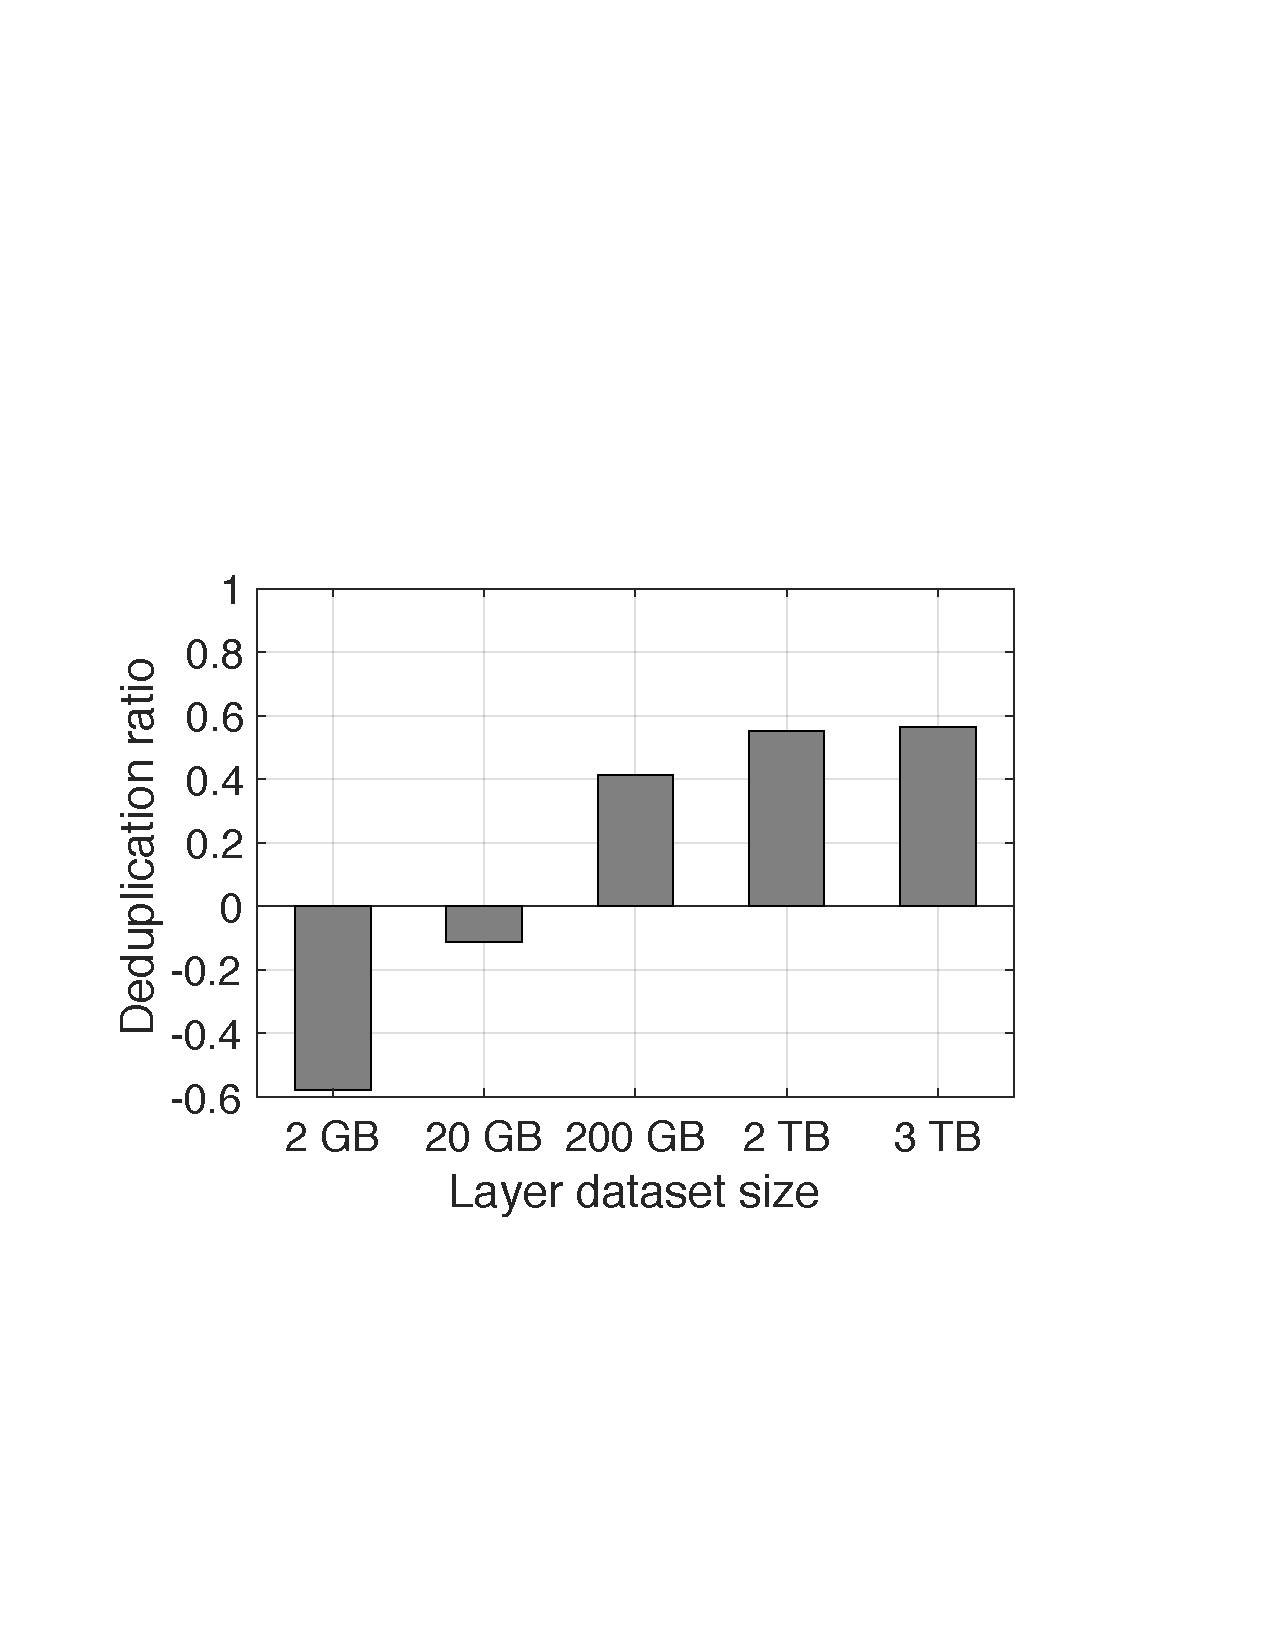
\includegraphics[width=1\textwidth]{graphs/dedup_vs_compression.pdf}
%			\caption{File-level deduplication vs. compression efficiency.}
%		%	\vspace{-3pt}
%			\label{fig:cacheefficiency}
%		\end{minipage}
%			\begin{minipage}{0.38\linewidth}
%				\centering
%				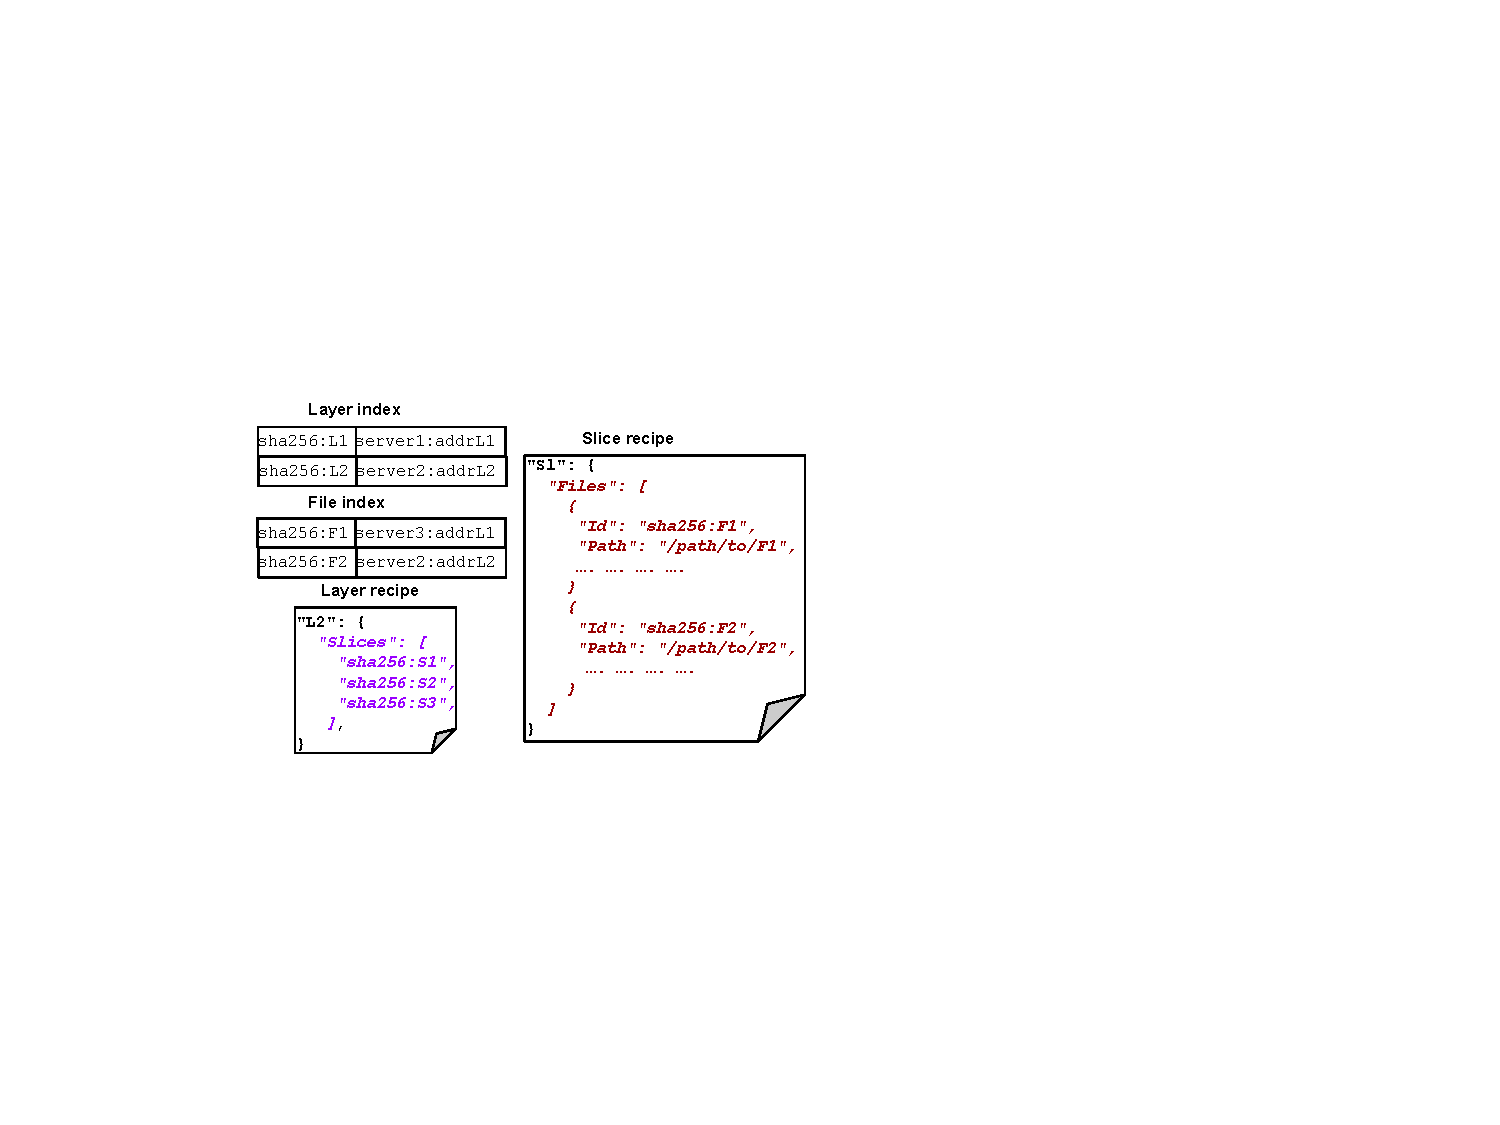
\includegraphics[width=1\textwidth]{graphs/sift-metadata.pdf}
%				\caption{Metadata for deduplication.}
%				%	\vspace{-3pt}
%				\label{fig:sift-metadata}
%			\end{minipage}
%		\begin{minipage}{0.38\linewidth}
%			\centering
%			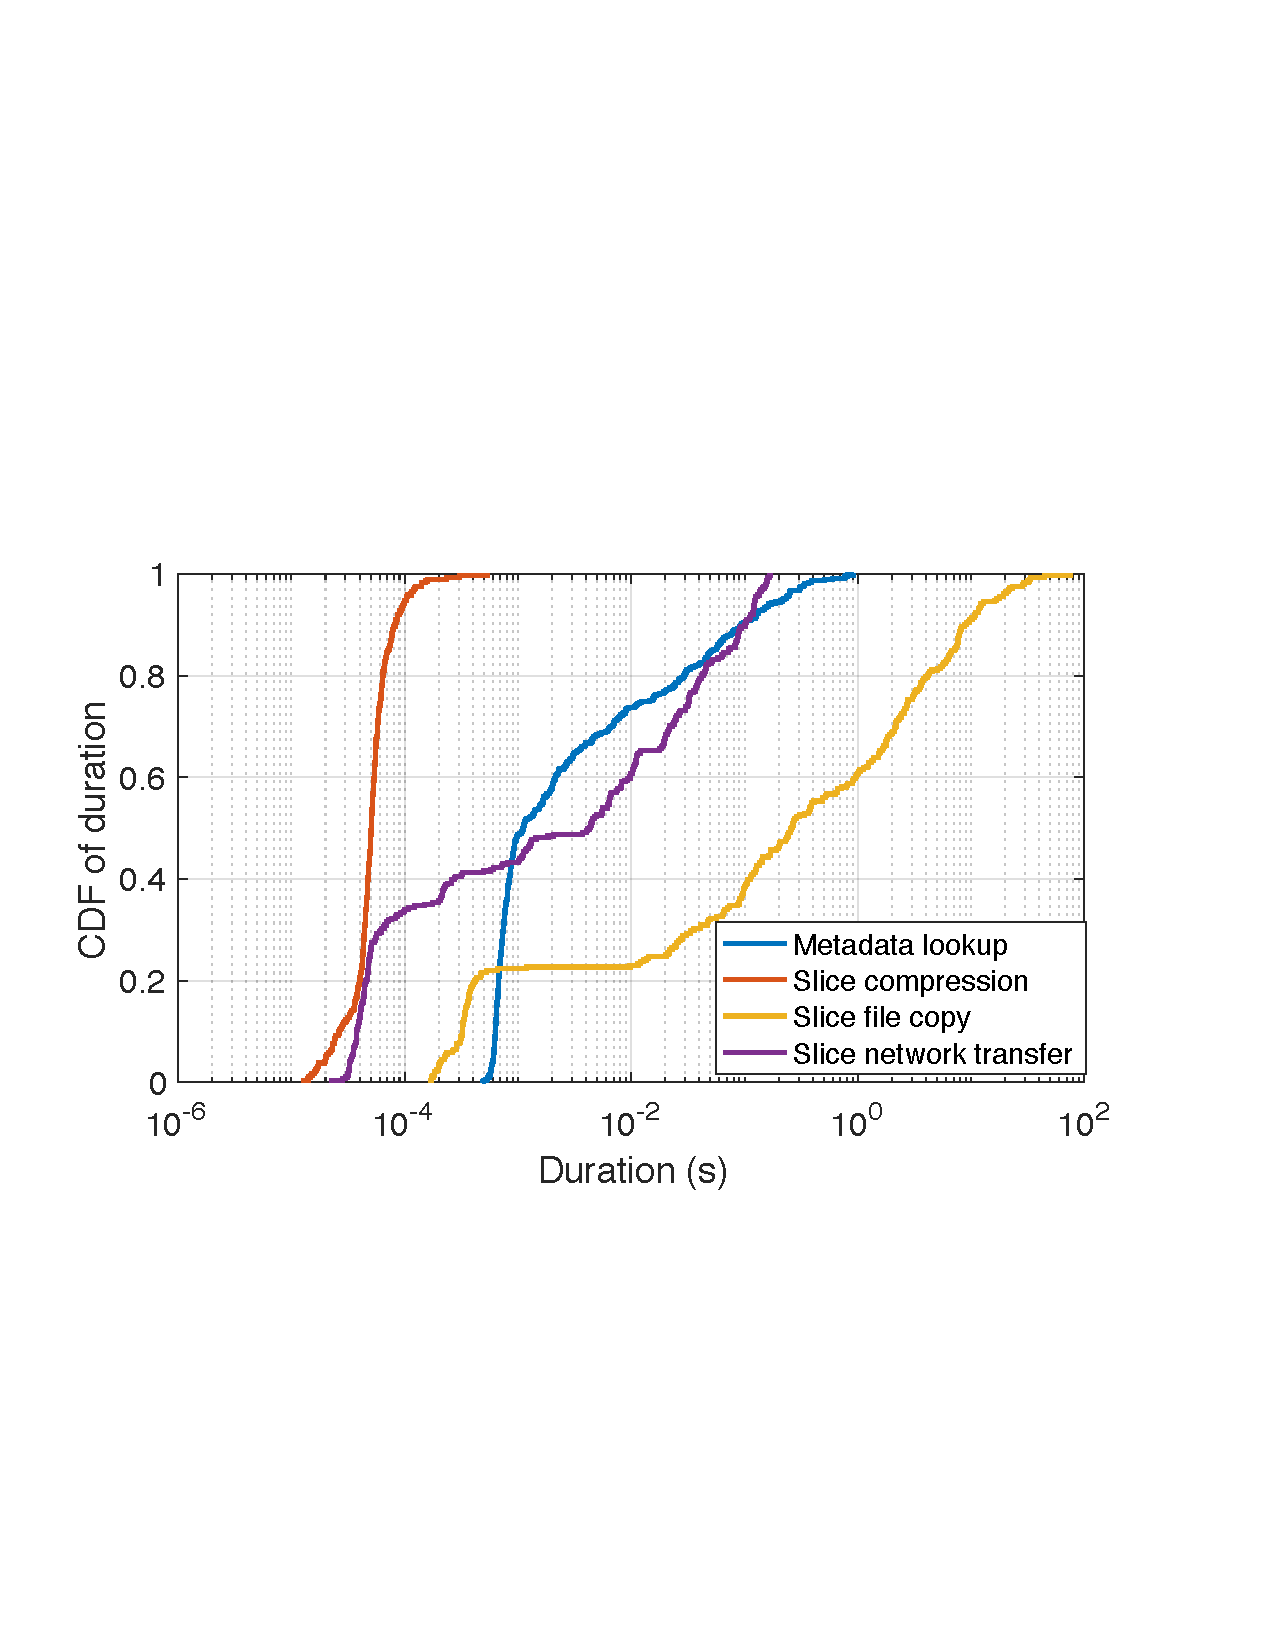
\includegraphics[width=1\textwidth]{graphs/restoring-breakdowns.pdf}
%			\caption{Breakdown of slice restoring time.}
%			%	\vspace{-3pt}
%			\label{fig:slice-restoring-breakdown}
%		\end{minipage}
%\end{figure*}

\begin{figure}[t]
	\centering
	\centering
	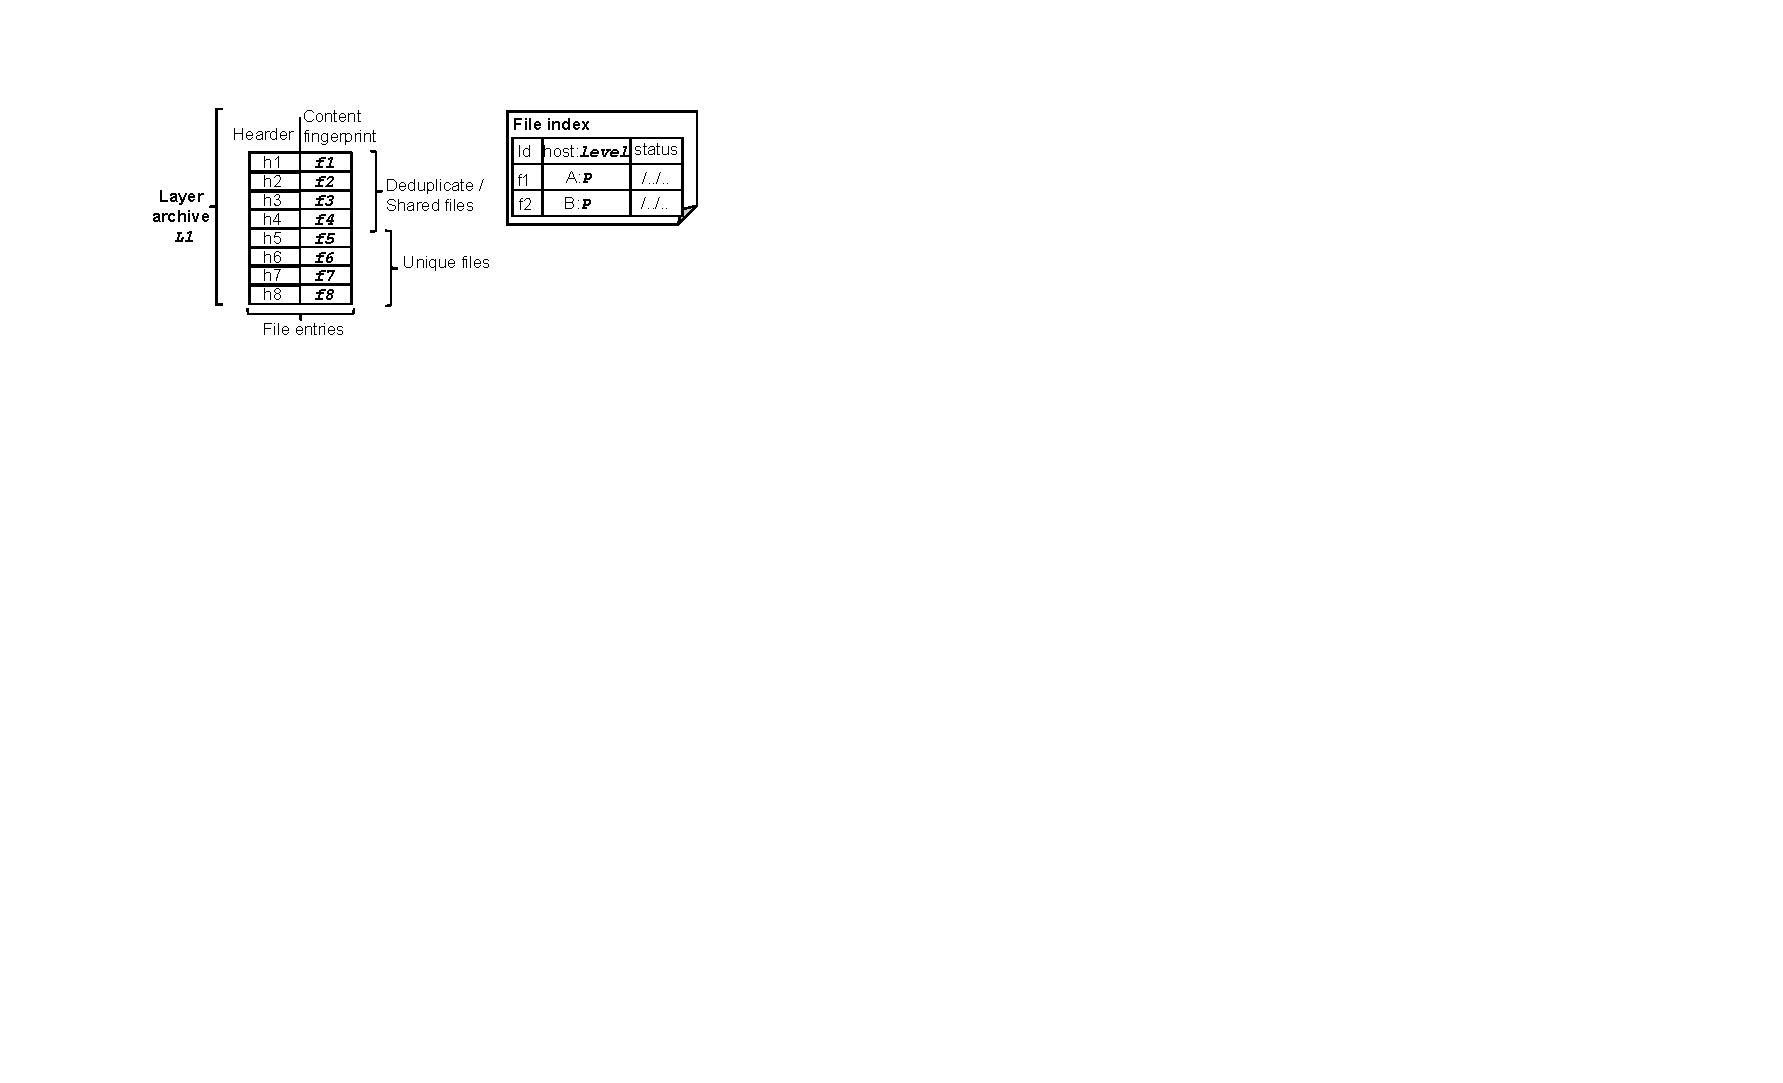
\includegraphics[width=0.45\textwidth]{graphs/sys-architecture-put-layer.pdf}
	\caption{Layer deduplication. \LR{Typo: ``Hearder'' should be ``Header''}}
	\label{fig:dedup-partition}
\end{figure}



%\begin{figure}[t]
%	\centering
%	\begin{minipage}{0.26\textwidth}
%		\centering
%		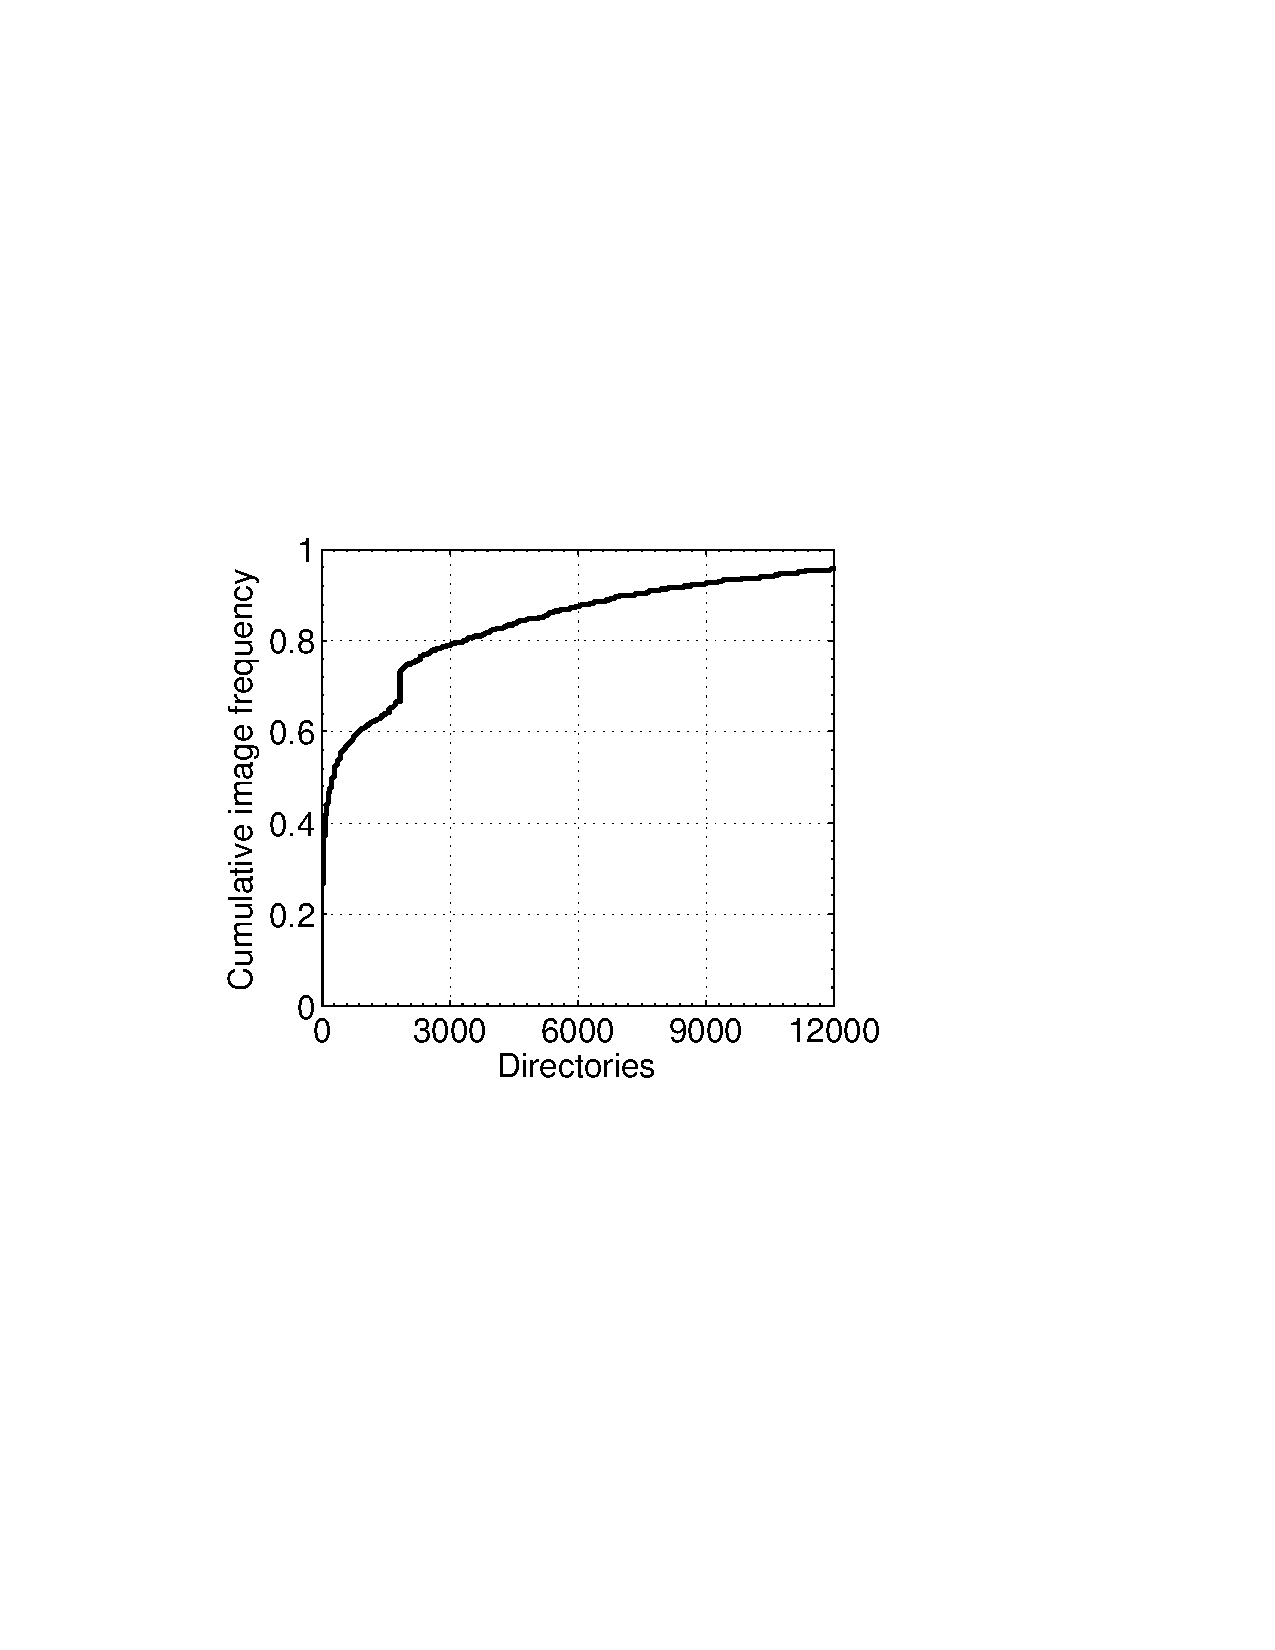
\includegraphics[width=1\textwidth]{graphs/dir.pdf}
%		\caption{CDF of images by\newline directories}
%		\label{fig-dir}
%	\end{minipage}%
%	\begin{minipage}{0.24\textwidth}
%		\centering
%		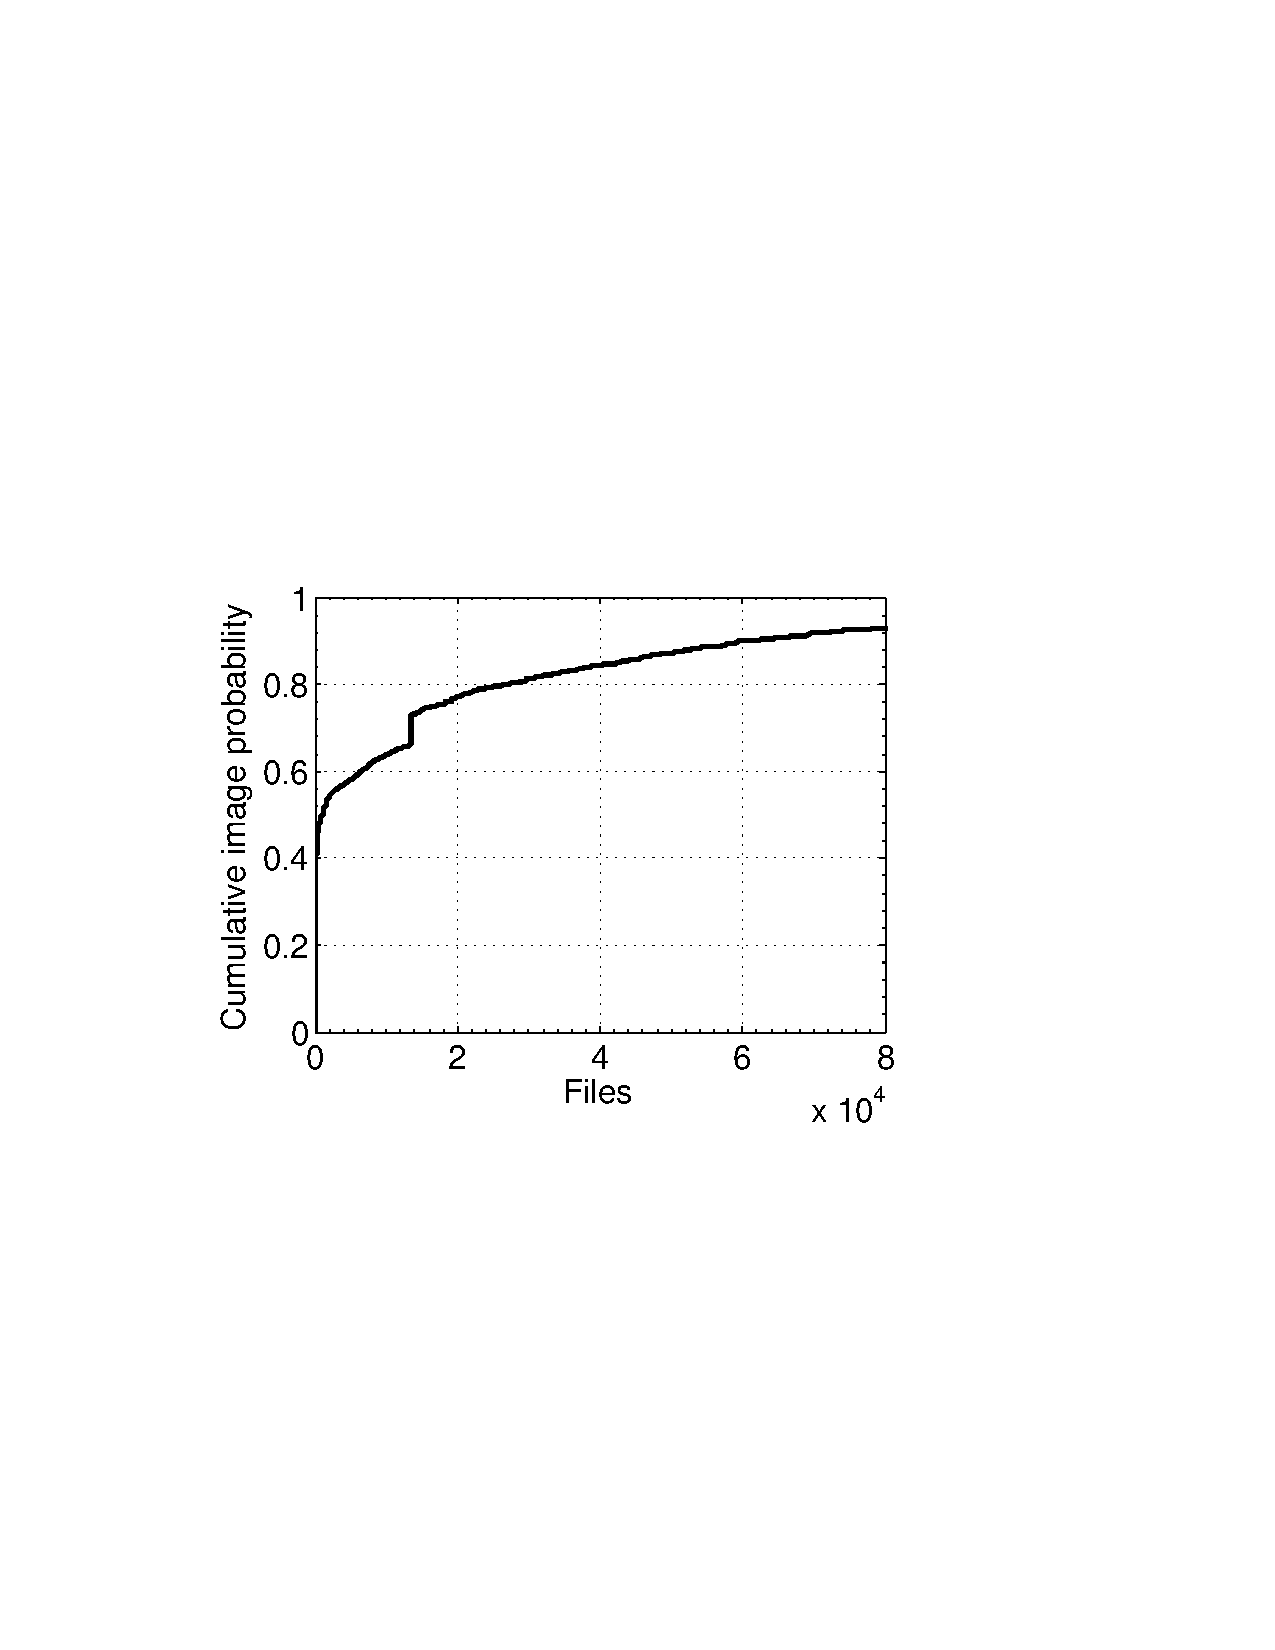
\includegraphics[width=1\textwidth]{graphs/file.pdf}
%		\caption{CDF of images by files}
%		\label{fig-file}
%	\end{minipage}
%\end{figure}

%\begin{figure}[htbp] 
%	\begin{minipage}{0.5\linewidth} 
%		\centering 
%		\includegraphics{circle} 
%		\caption{A Circle} 
%		\label{fig:circle} 
%	\end{minipage}% 
%	\begin{minipage}{0.5\linewidth} 
%		\centering 
%		\includegraphics{rectangle} 
%		\caption{A Rectangle} 
%		\label{fig:rectangle} 
%	\end{minipage} 
%\end{figure}

%\begin{figure}[t]
	\centering
%		\begin{minipage}{0.23\textwidth}
%			\centering
%			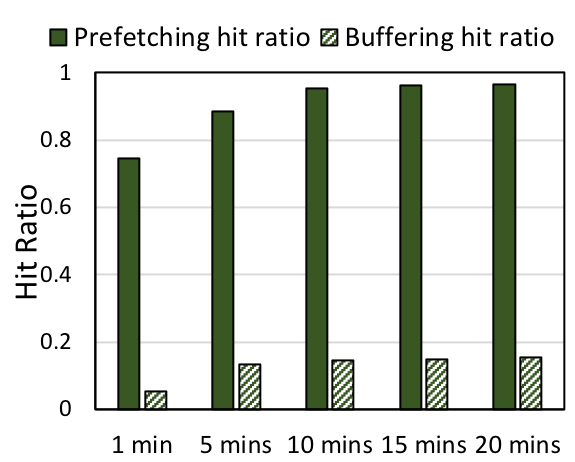
\includegraphics[width=1\textwidth]{graphs/evaluation_hitratios.png}
%			\caption{Hit ratio.}
%			\label{fig:hitratio}
%		\end{minipage}
	%	\begin{minipage}{0.25\textwidth}
			\centering
			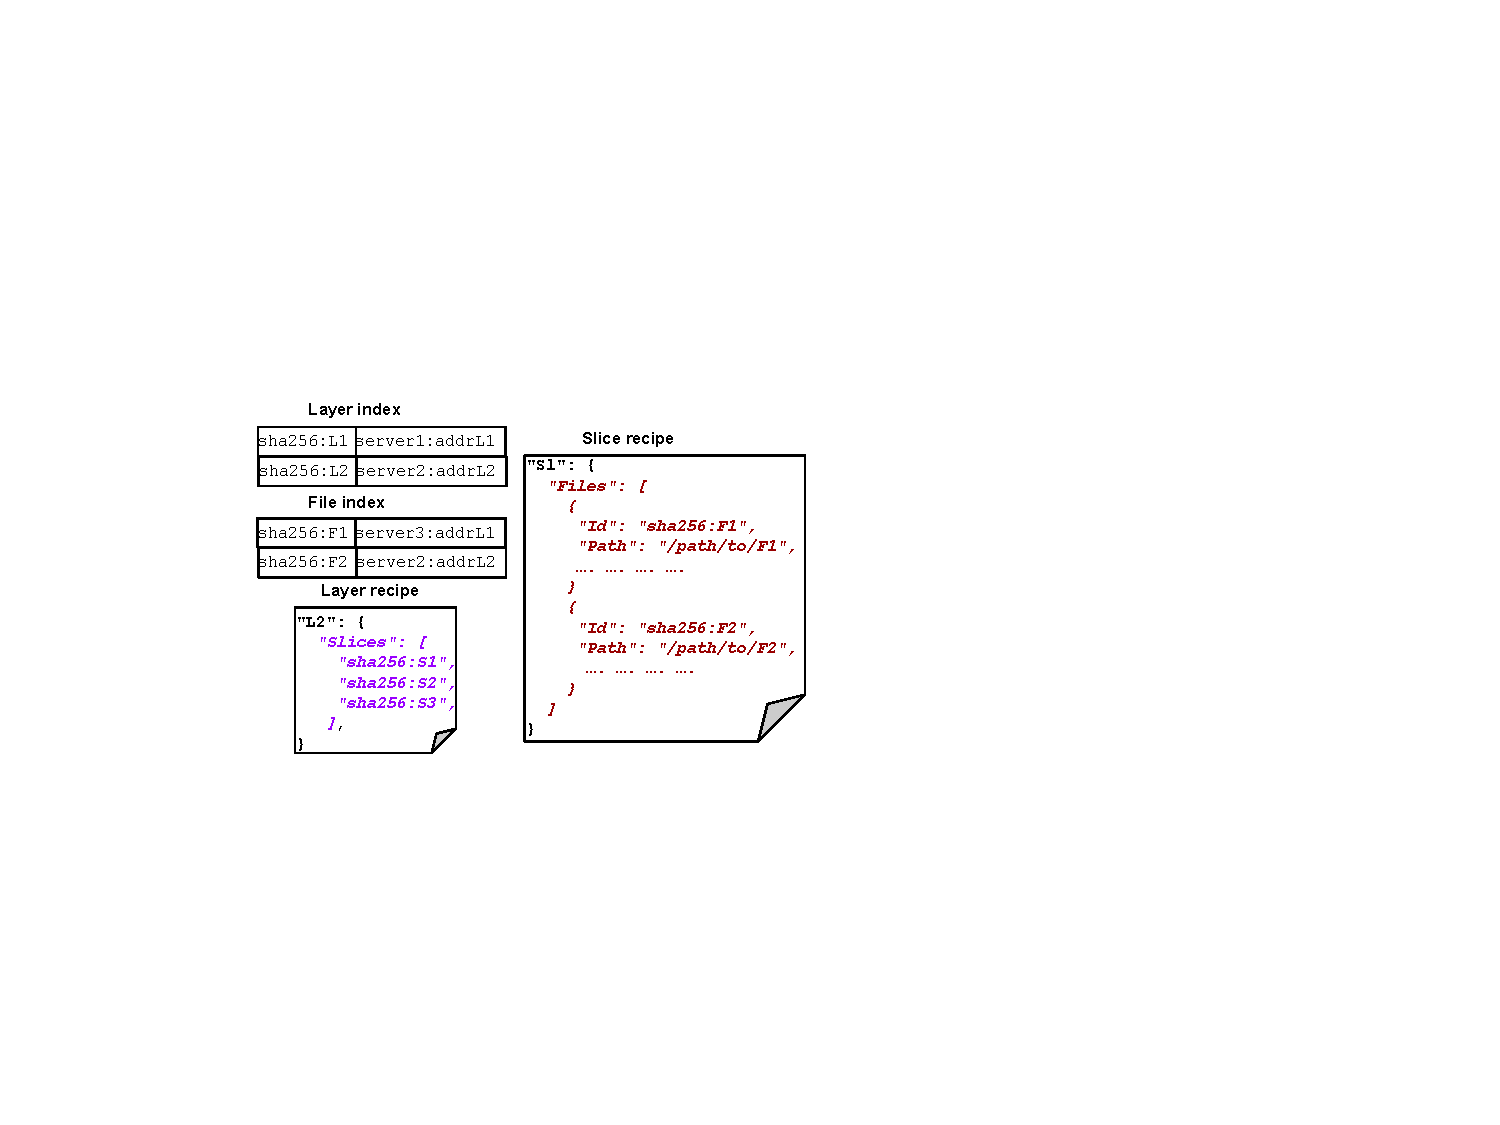
\includegraphics[width=0.4\textwidth]{graphs/sift-metadata.pdf}
			\caption{Metadata for deduplication.}
			%\vspace{-3pt}
			\label{fig:sift-metadata}
	%	\end{minipage}
\end{figure}
\paragraph{File-level deduplication}
%\LR{Is the following just how the .tar format is structured or are we doing anything
%additional to the headers and the content? If not, we should just mention that this is
%how tar is creating archives.}
%
%As shown in Figure~\ref{fig:dedup-partition},
Following the staging area, \sysname
uncompresses the layer and passes the decompressed tar file to the deduplication process.
%In this process, 
%the layer tarball is first decompressed into a \textbf{layer tar archive}~\cite{xxx}.
%Algorithm~\ref{alg:dedup-partition} details layer deduplication and partitioning. 
%After layer decompression, 
Each file entry in the archive is represented as a \emph{file header} and the associated
\emph{file content}~\cite{basictar}.
The file header contains metadata such as file name, path, size, mode, owner information, etc.
%
%and is needed to correctly rebuild the \emph{file header} for 
%the associated file entry in the restoring layer archive.
%
\sysname records every file header in slice recipes (described below)
to be able to correctly restore the complete layer archive later.
%
%
%##### need to record all files in the tar archive, not just unique files' header but also the deduplicated
%files'headers. otherwise, how do you restore a complete tar achieve?????
%
\sysname computes the file Id for each file by hashing the file content and 
checks, whether the file Id is already present in the file index.
If the file Id is already stored, the file content will be discarded. 
Otherwise, it will be saved physically in the D-server's file store and 
the file Id is recorded in the file index.%
% As shown in Figure~\ref{fig:replication-partition},
The file index maps different file Ids to the physical file replicas stored
on different D-servers.
%represented as a file location and a file size.
%File location is denoted as 
%Besides, each file Id in the file index is also mapped to its \emph{host address} with the associated \textbf{backup level}.
%Backup level denotes whether the host stores a primary backup file replica (i.e., \texttt{P}) or the $n^{th}$ backup replica (ie., \texttt{B}\emph{n}) detailed as follows.
%detailed as following.

%\LR{Here, we need to explain in more detail, what exactly a slice is (just a collection of headers?),
%how a header is linked to its file content, and how files/headers are linked to layers (through layer
%recipe? We should also talk a little bit about our metadata overhead here.}

\paragraph{Unique file replication}
%
%Note that, layer deduplication process only deduplicates regular files., 
%
Next,
\sysname replicates and distributes unique file replicas across D-servers.
%Hence, the layer partitions on D-servers can be used to restore a \emph{slice} of layer in parallel.
%To speedup layer restoring process,
%\sysname distributes file replicas and 
%in a way such that
%each server is able to rebuild an $\sim$equal-sized slice of the layer from its local file store.
%
%As mentioned earlier, \sysname records every file header from a layer tar archive.
%Sift will hold on to the file headers from tar archive to be included as part of the slice recipe.% \Subil{The previous sentence seems to indicate that the header-contentpointer pairs are stored in the D-server. But they are only stored in the metadata database as part of the slice recipe, right?}
%\NZ{yes}
The headers and content pointers of all the files, in a given D-server, that belong to a particular layer are included in that D-server's \emph{slice recipe} for that layer.
%(see Figure~\ref{fig:replication-partition}). 
%After unique file replication and layer partitioning,
After file replication, \sysname adds the new slice recipes to the metadata database.
%A slice recipe represents a layer slice and is used to construct a
%\emph{partial layer archive}.

\sysname also creates a \emph{layer recipe} for the uploaded layer and stores it in the metadata database.
%as shown in Figure~\ref{fig:replication-partition}.
The layer recipe records all the D-servers that store slices for that layer and which can act
as \emph{restoring workers}. When a layer needs to be reconstructed,
one worker is selected as the \emph{restoring master}, responsible 
for gathering all slices and rebuilding the layer~(see~\S\ref{sec:restore-desgin}).

Figure~\ref{fig:replication-partition} demonstrates how Sift pipeline operates.
The example assumes B-mode 1 with 3-way replication, i.e. each unique file has two replicas distributed
on two different D-servers.
The files $f1$, $f2$, and $f3$ are already stored in \sysname,
and $f1'$, $f2'$, and $f3'$ are their corresponding backup replicas.
Layer $L1$ is being pushed and contains files $f1$, $f2$, $f3$, $f4$, $f5$, and $f6$. 
%is decompressed and \emph{file-level deduplicated}.
$f1$, $f2$, and $f3$ are \emph{shared files} by $L1$ and other layers, and hence,
are discarded during file-level deduplication.
%\emph{f1, f2,} and \emph{f3} are shared by \emph{L1} and other layers, denoted as \textbf{shared files}.
The unique files $f4$, $f5$ and $f6$ are added to the system and
replicated to D-servers $A$, $B$, and $C$.
%We describe how the target servers are chosen later in this section.

After replication, server $B$ contains $f2$, $f5$, $f1'$, and $f4'$. Together
$f2$ and $f5$ form the \emph{primary slice} of $L1$, denoted as $L1::A::P$.
This slice Id contains the layer Id the slices belongs to ($L1$), the node, which
stores the slice ($A$) and the backup level ($P$ for primary).
%\todo{explain this notation}.
%\NZ{This slice Id contains the layer Id it belongs, the host server, and the backup level of this slice.
%This slice Id notation largely simplifies layer recipe and facilitate layer restoring.
%The restoring master only needs to fetch a small layer recipe, get the restoring workers,
% and decide which backup level slices are needed for layer restoring.
% After that, the master sends out simple layer restoring instructions to the workers.
% The layer restoring instruction only contains the layer Id and the backup level.
%The workers will generate a slice Id by using the layer Id and backup level
%along with its own address, which holds the slice stored locally.}
%
%shared file replica \emph{f2} and 
%unique file replica \emph{f5} stored on \emph{B} comprise a slice of \emph{L1},
%denoted as a \textbf{primary slice} of \emph{L1} (ie., \emph{L1::A::P}).
The two backup file replicas 
$f1'$ and $f4'$ on $B$ form the \emph{backup slice} $L1::B::B$.
During layer restoring, $L1$ can be restored by using any combination of primary and backup slices
to achieve maximum parallelism.
%
%\LR{Why are \emph{f4'} and \emph{f8'} only a backup slice?}
%\LR{Instead of putting the fX in emph environments, we should use math mode and put numbers in the index, e.g.
%$f_{4}'$.}

%=======
%After discarding duplicate files
%, the deduplication process distributes the layer's remaining files across different registry servers
%so that each server is able to build an $\sim$equal-sized % subil: is the \sim necessary?
% slice of the layer from its local file store when needed.
% We define the collection of files that belong to a layer as a \emph{slice} of that layer stored on the registry server. 
%A server stores slices for many layers, and a layer is composed of slices stored on multiple servers, which allows restoring a layer in parallel. 
%Finally, \sysname will add slice recipes and layer recipe to metadata database as shown in Figure~\ref{fig:dedup-partition}.
%
%Figure~\ref{fig:replication-partition} shows an example of file replication and layer partition.
%Each file has two replicas distributed on different servers,
%\emph{r1, r2, r3,} and \emph{r4} are four primary file replicas that were already stored in the system.
%and \emph{r1', r2', r3',} and \emph{r4'} are their associated backup file replicas. 
%A layer \emph{L} that contains files \emph{r1, r2, r3, r4, r5, r6, r7,} and \emph{r8} is pushed.
%Files \emph{r1, r2, r3,} and \emph{r4} are deduplicated
%while new files
%\emph{r5, r6, r7,} and \emph{r8} will be added to the system, 
%As shown, \emph{r5, r6, r7,} and \emph{r8} are replicated and distributed to registry \emph{A, B, C,} and \emph{D} 
%as primary file replicas and backup file replicas.
%Consequently,
%primary file replicas \emph{r1} and \emph{r5} stored on registry \emph{A} comprise one of layer \emph{L'}s slices, 
%denoted as \textbf{primary slice}:
%\emph{layerid:A}.
%The two backup file replicas \emph{r4'} and \emph{r8'} stored on registry \emph{A} comprise a \textbf{backup slice} for the primary slice stored 
%on registry \emph{D} (i.e., \emph{r4} and \emph{r8}).
%>>>>>>> ab86d0a4767bfcfcbb58baf9bd7b2e81e54d7e51

%primary file replicas
\begin{figure}[t]
	\centering
	\centering
	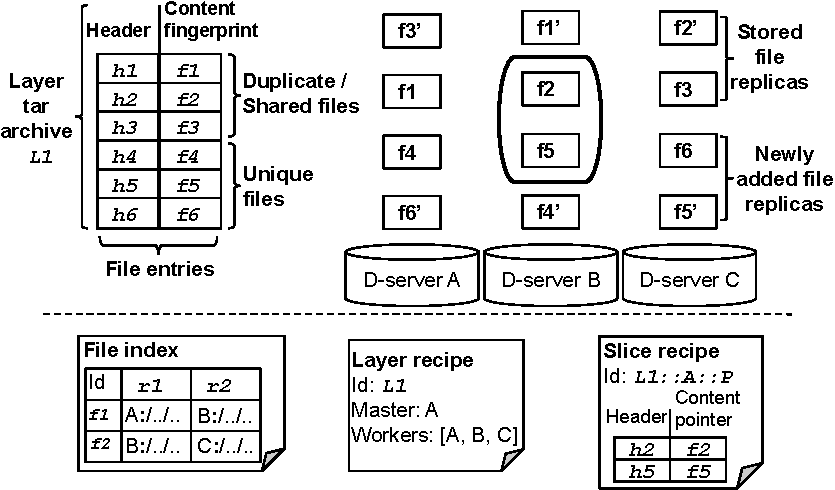
\includegraphics[width=\columnwidth]{graphs/replication.pdf}
	\caption{Layer dedup, replication, and partitioning.}
	\label{fig:replication-partition}
\end{figure}

%\begin{algorithm}
\scriptsize 
	\caption{Layer deduplication and partitioning}
	\label{alg:dedup-partition}
	\KwIn{\\	
			$FileIndex$: File index. \\
	}

	\KwOut{\\
			$LayerRecipe$: Layer recipe for layer $L$.\\
			$SliceRecipes$: Slice recipes for layer $L$' slices.\\
	}

	archive $\leftarrow$ \texttt{Decompress} layer $L$ \\

	\ForEach{header, content in archive} 
	{ 
		Id $\leftarrow$ \texttt{Hash} content \\
		%destHeader $\leftarrow$ header \\
		\eIf{ Id in FileIndex}{
			host  $\leftarrow$ $FileIndex$[Id].host \\
			src $\leftarrow$ $FileIndex$[Id].header \\
			{\tiny\texttt{/* SliceRecipe is identified by `layerid::host'}}
			SliceRecipe[$L::host$] $\leftarrow$  \texttt{Add} (header, src) \\
			{\tiny\texttt{/* Skip redundant file.  }}\\
		}{
			{\tiny\texttt{/* create file with content in file store.  }}\\
			file $\leftarrow$ \texttt{Create and write} content \\
			src $\leftarrow$ \texttt{Stat} file \\
			entries $\leftarrow$ (header, src)  \\
		}
	}
	
	\Do{entries}{
		{\tiny\texttt{/* get file entry with maximum file size. }}\\
		maxFile $\leftarrow$ \texttt{Max} entries \\
		{\tiny\texttt{/* get smallest slice. }}\\
		minSlice $\leftarrow$ \texttt{Min} SliceRecipes \\
		{\tiny\texttt{/* assign biggest file to smallest slice. }}\\
		minSlice $\leftarrow$ \texttt{Add} maxFile \\
		{\tiny\texttt{/* Set maxFile to FileIndex}}\\
		{\tiny\texttt{/* Remove maxFile from entries. }}\\
	}
	{\tiny\texttt{/* Send slices.}}\\
	{\tiny\texttt{/* Set SliceRecipes.}}\\
	{\tiny\texttt{/* Include all slices' hosts to workers.}}\\
	{\tiny\texttt{/* Select biggest slice' host as master.}}\\
	{\tiny\texttt{/* Set LayerRecipe.}}\\
	
	
		
\end{algorithm}




%<<<<<<< HEAD
%Then, the process sends slices to the corresponding registries.
%Slice is identified by a simple combination of the layer id and its host address 
%with the associated backup level,
%denoted as $layerid::host::backuplevel$. % as shown in Algorithm~\ref{alg:dedup-partition}.
%As shown in Figure~\ref{fig:replication-partition},
%the primary slice stored on \emph{A} is denoted as \emph{L::}\emph{A::}\texttt{P}
%while the rest backup slice is denoted as \emph{L::}\emph{A::}\texttt{B2}.

%=======
%Algorithm~\ref{alg:dedup-partition} details layer deduplication and partitioning algorithm.
%After layer decompression, 
%each file entry in the layer archive % subil: what is the layer archive referring to?
% is represented as a \textbf{file header} and a \textbf{file content}.
%The file header contains the file name, path, size, mode, owner information, etc. % subil: should elaborate on structure of the header, how is it constructed?
%The file header is needed to rebuild the \emph{file header} % subil: how are the two file headers different?
%for 
%the associated file entry in the layer archive.
%
%%During layer deduplication process,
%\sysname records each file entry's file header and 
%calculates the file id by hashing the file content.
%As mentioned earlier, the file index maps a \emph{file id} to its associated physical file that is stored in the file store.
%To address a physical file,
%each file id in the file index holds its 
%%denoted by a combination of its 
%\emph{host address} and \textbf{file status} of the physical file which mainly contains file name, path, and size.
%As shown in Algorithm~\ref{alg:dedup-partition}, 
%if a file's id already exists in file index (i.e. it's present in a registry server), 
%this file will be added to its host's corresponding slice for that layer. 
%Otherwise,
%\sysname stores the file content as a physical file in the file store
%and retrieves the file status of the physical file.
%The file index is updated accordingly.
%
%The slice recipe is identified by a simple combination of the layer id and its host registry address,
%denoted as $layerid::host$ as shown in Algorithm~\ref{alg:dedup-partition}.
%A slice recipe represents a layer partition and
%is used to construct a partial layer,
%>>>>>>> ab86d0a4767bfcfcbb58baf9bd7b2e81e54d7e51
%which
%records each file entry' $header$ in the layer archive partition and 
%its corresponding physical file's status . 
%In this case, 
%each file is represented as a $header$ in the layer archive and
%its corresponding physical file's status $src$. 
%
%During layer deduplication process,
%After unpacking the layer archive, 
%
%Note that destHeader can be used to rebuild the \textbf{file header} for 
%associated file entry in the layer archive.
%
 %its host' slice
%to get identical files' server addresses.

%\LR{The following needs to be reformulated to be more clear.}
%
\paragraph{Layer partitioning}
To improve reconstruction times, it is important that different layer slices
are equally sized and evenly distributed across D-servers.
%The example in Figure~\ref{fig:replication-partition}
%shows such a perfect scenario, in which the files of layer $L1$ are evenly partitioned across all D-servers.
%since its shared files and unique files are evenly distributed to D-servers. 
%However, in general, it is not straightforward to evenly distribute shared files for different
%layers as their placement is fixed by the first layer, which was pushed to the registry that
%contained these files.
%\LR{Provide more details. Why is that so? Is this assuming consistent hashing?}
%\NZ{Let's consider an empty storage system, the first layer can be easily evenly partitioned
% to servers because no shared files are stored.
%After the first layer is partitioned and stored,
%consider that the second layer is pushed,
%the second layer has some same files with the first layer and
%these shared files are already distributed to servers.
%These shared files are distributed in a way such that the first layer can be evenly partitioned.
%But they might not be evenly distributed for the second layer because
%when we distribute files for first layer we dont know the subsequent layers and
%we dont know which files will be shared with the subsequent layers.
%So the shared files' layout will affect the subsequent layers' partition.}
%
%To evenly distribute and partition a layer's unique and shared files
%, shared and unique files,
%
%To distribute the newly added unique files' primary replicas,
To achieve this, \sysname employs a greedy packing algorithm.
%, which is constrained by  with shared file constraints.
%distribute the newly added unique files in a way such that
%each D-server stores relatively equal-sized slice for the layer.
%\LR{What exactly is meant by `shared file constraints'. Can we explain a bit more?}
%\NZ{It means before partition the layer, some of its containing files (shared files)
%are already allocated to the servers.
%We dont want to migrate those files to make all its containing files evenly distributed.
%So I called it a constrain.
%It means when we partition layers, we maintain its containing shared files that are already allocated
%and stored on servers as it is. 
%Through only distribute the newly added unique files,
%we achieve a relatively even partition for a layer.}
%
Consider first the simpler case in which each file only has
a single replica. During layer partitioning, \sysname does not migrate shared files that already
have been stored on D-servers to reduce I/O overhead.
%
%\LR{The following is unclear, why does \sysname partition shared files for $L1$? Aren't they already there?}
%\NZ{I think it's allocating not partitioning.}
%
%\sysname first partitions $L1$ shared files to their host servers.
%\sysname first determines the location of $L1$'s shared files in the cluster.
%For example, in Figure~\ref{fig:replication-partition}, shared files $f1$, $f2$, and $f3$ are located
%on D-servers $A$, $B$ and $C$ respectively. It then computes the total size of the shared files
%for each affected D-servers.
\sysname first computes the total size of the layer's existing shared files for each D-server (this could
potentially be 0 if a D-server does not store any shared files for the layer).
Next, \sysname 
%starts to assign unique files to D-servers following a greedy packing strategy.
assigns the biggest unique file to the smallest partition until all the unique files are assigned.
%In the example, the shared files are evenly partitioned to all three D-servers,
%and hence, the three newly added unique files are also evenly assigned to the three servers.
%Otherwise, the biggest unique files will be assigned to the smallest partitions.
%\LR{As a general note, it seems like we generate quite a bit of metadata to keep track
%of the slices etc. Are we planning to evaluate how much metadata we generate?}
%\LR{Here, we need to talk about how we are planning to address the problem of metadata management as
%we are manually assigning files to servers and hence, have to store the location of each file in an index.
%How do we scale? What if we are dealing with billions of files?}
%\NZ{We just add a server address for each file Id in the file index.
%As shown in implementation section,
%we store the unique files as: ‘rootdir/docker/registry/v2/uniquefiles/sha256/
% <first two hex bytes of file digest> /<hex file diges>t’ so that given a file digest, 
% we can build the file path to save metadata information.}
%Finally, \sysname updates the file index with the newly added unique files.

%\LR{The following is unclear and needs a better explanation. Are the new primary replicas
%assigned to servers which do not yet store shared files for the new layer? What if all
%servers already store at least one shared file for the layer? How are the backup replica
%servers picked?
%}
%\NZ{The shared files also have primary replica and backup replicas.
%Simply, we distributed the primary replica of newly added unique files
%according to the distribution of primary replicas of shared files.
%And we distributed the secondary replicas of newly added unique files
%according to the distribution of secondary replicas of shared files to maintain a relatively even partition.
%Moreover, we also make sure that the secondary replicas of a newly added unique file
%is not stored on the same server with its primary replica.
%So when we distribute the secondary replicas, we need to consider the 
%secondary replicas of shared files and the previously allocated primary replicas.
%}
%
In the case where a file has more than one replica, \sysname performs the
above described partitioning \emph{per replica}. That means that it first assigns
the primary replicas of the new unique files to D-servers according
to the location of the primary replicas of the existing shared files. It then assigns the secondary
replicas according to the location of the existing secondary replicas and so on.
Additionally, \sysname also ensures that two replicas of the same file are never
placed on the same node.

%Next, we consider the case that each file has multiple replicas. The file
%index contains the location of the primary and backup replicas for each shared file.
%%For each shared file, its file Id points to multiple file replicas in the file index as
%%shown in Figure~\ref{fig:dedup-partition}.
%When adding new unique files, \sysname first distribute the files
%according to the shared files' primary file replicas' partitions. After that,
%\sysname assigns the replicas of unique files onto different servers with their primary
%replicas.

%After layer partition,.
%All the primary slices' hosts are denoted as layer restoring \textbf{primary workers}. 
%Next, \sysname stores slice recipes in metadata database after successfully
%sending slices to their corresponding workers.
%\sysname selects the biggest slice' host as layer restoring \textbf{primary master}.
%Layer recipe records the primary workers and master information for layer restoring.
%After that, \sysname~distributes primary slices' corresponding backup slices.
%Their hosts are denoted as \textbf{backup workers}.
%Finally, \sysname stores layer recipe in metadata database.
%Layer recipe 

%Here, we use the metadata database as a distributed lock for file index.
%File index sets a file id to hold  only if the file id does not exists.

%it uses a weighted round robin algorithm to distribute newly added 
%unique files to the registry cluster. These servers that already contains this layer's identical files
%are assigned a lower weight. 
%This is to ensue that different servers maintain same amount of files that are needed to restoring equal sized 
%slices for this layer.
%Deduplication process also 
%updates the \emph{file index} with the newly added unique files' fingerprints and host addresses.   
%Then, it calculates the slice fingerprints and creates a slice recipe for each slice.
%Slice recipe contains partial of the layer tarball's directory tree structure, file fingerprints, file name along with file path in the tarball, and file metadata information 
%(such as permissions and creation date), which are needed for restoring a slice for the layer. 

%After that
%After removing the duplicate files,
%Then, it
%distributes the \emph{deduplicated slices} evenly to the registry cluster by using round-robin, and,
%In the end, deduplication process creates a layer recipe which contains its slices' fingerprints and 
%based on layer recipe, it updates image manifests.
%The layer's tarball and file duplicates are removed after deduplication.

%<<<<<<< HEAD
%\subsection{Layer restoring}
%\label{sec:restore-design}
%%\paragraph{Parallel slice restoring}
%%\label{subsubsec:slice-restoring}
%
%

\begin{figure}[t]
	\centering
	\centering
	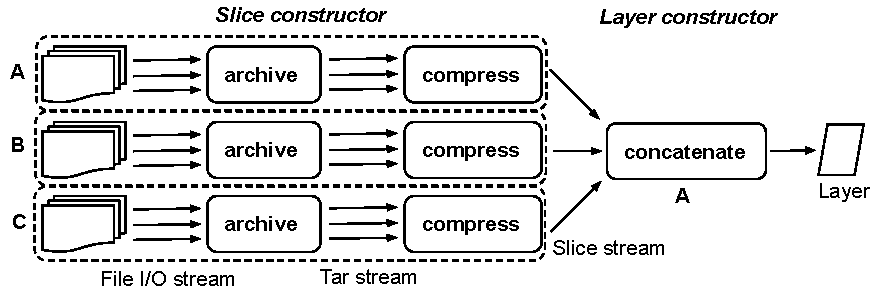
\includegraphics[width=\columnwidth]{graphs/sift-layer-construct-new.pdf}
	\caption{Parallel streaming layer construction.}
	\label{fig:construct}
\end{figure}


%
%When a~\texttt{pull} layer request is received and its associated 
%P-servers fail, 
%\sysname will first search layer diskcache on D-servers.
%If not found,
%\sysname will rebuild the layer from file store according to its layer recipe. 
%%the \dedupname~system 
%%first prepares a directory structure for the slice, based on the slice recipe.
%%Then, it copies the files into the directory tree.
%%Next, it compresses the slice's directory tree into a slice tarball,
%%and directly sends it back to the client.
%
%\paragraph{Parallel layer construction}
%
%When a~\texttt{pull} layer request is received, 
%\sysname will update \emph{ULmap}. 
%ULmap records user access status,
%which maps a \textbf{user id} to its accessed layers with its corresponding access count,
%where user id is defined as client request address.
%
%Upon a \texttt{pull} layer request fails on P-servers,
%\sysname initiates a layer restoring process on D-servers for it.
%The process has two parts: slice constructor and layer constructor.
%Figure~\ref{fig:restoring} shows an example of parallel layer restoring when a \texttt{pull} layer request failure happens.
%First, 
%layer constructor fetches the layer recipe from metadata database.
%As shown in $L1$'s layer recipe, 
%the primary restoring workers contains registry $A$, $B$, and $C$.
%Since registry $A$ is the primary restoring master,
%\emph{A} sends ``\texttt{Get primary slice}" requests to its peer workers: $B$ and $C$.
%After a \texttt{Get primary slice} request is received, 
%$B$ and $C$ start primary slice construction and return a primary slice back to $A$ respectively.
%Meanwhile $A$ instructs local slice constructor to rebuild a primary slice for $L1$.
%Slice constructor first gets its associate slice recipe (``$L1::P:A$") from metadata database 
%keyed by a combination of  layer id, slice type (i.e., primary $P$ or backup $B \#$) and registry address.
%Then, based on slice recipe,
%slice constructor fetches files pointed by $Srcs$
%and builds a slice archive.
%After receiving all slices, layer constructor concatenates them into a compressed layer
%and sends back the client. 
%
%\paragraph{Streaming layer construction}
%Figure~\ref{fig:construct} details the stateless streaming layer construction process.
%First, slice constructor loads file in parallel from file store based on the slice recipe.
%Each file is written to an archive buffer asynchronously.
%Before writing file content to the archive buffer, slice constructor first builds and writes its
%associated 
%file header into the archive buffer according to the slice recipe. 
%After archiving all the files in the slice,
%the archive buffer will be divided into few chunks and compressed in parallel,
%then concatenated into a single compressed slice stream.
%Through network transfer, multiple slice streams will be concatenated into a single layer.
%No intermediate file will be created or stored on disk. % subil: whoa!
%\sysname uses a small file inmemory cache to reduce file I/Os. 
%File cache uses Adaptive Replacement(ARC)~\cite{xxx}.
%
%%headers according to $Dests$,
%%after that it writes file contents into the archive
% 
%%Slice restoring process has four suboperations: 
%%slice recipe lookup,
%%slice file copying,
%%slice compression, and
%%slice network transfer. 
%%To measure the overhead for each suboperation, 
%%we implemented layer deduplication and parallel slice
%%restoring on a 4-node registry cluster. 
%%We first warmup the cluster by pushing 200 layers to the cluster
%%and initiating layer deduplication process.
%%The layers were randomly selected from our layer dataset detailed in xxx limited to 50MB.
%%After finishing layer deduplication,
%%we sent 400 \texttt{pull slice} requests to the cluster with 10 \texttt{pull slice} requests issued at a time.
%%Figure~\ref{fig:slice-restoring-breakdown} shows the CDFs of the latencies for each suboperation.
%%We see that across the four suboperations,
%%the duration for slice compress is the shortest.
%%Slice compression only took less than 0.001 s because a slice is a smaller unit. 
%%The next shortest suboperation is network transfer since we pulled layer slice through Ethernet.
%%90\% of slice recipe lookups took less than 0.1 s while 
%%the highest slice recipe lookup duration almost reaches 0.8 s,
%%which is caused by high concurrent lookup requests 
%%%(note that we use redis to store metadata \NZ{use mongodb instead}).
%%The most time consuming suboperation is slice file copying, which involves 
%%copying all 
%%the files that belong to the slice to their destination directory based on the slice recipe.
%%Note that we implemented a thread pool on each registry server to read files in parallel
%%and write data in RAMdisk to reduce disk IOs.
%%40\%of slice file copying duration is greater than 1 s and 
%%10\% of slice file copying duration is higher than 10 s.
%%This is because bigger slices contains more files and requires more disk IOs.
%%The overhead of slice copying can be largely mitigated for a large-scale registry cluster
%%since the size of slice roughly equals to $S_{l}/N$, where $S_{l}$ denotes the layer size and $N$ is size of registry cluster.
%%However, it could be a bottleneck for slice restoring on a small-scale registry cluster.
%%%and slice file copying duration depends on slice size.
%%
%%%\begin{algorithm}
\scriptsize 
	\caption{File cache assisted slice restoring}
	\label{alg:file-cache}
	\KwIn{\\
		$\theta_{rsfc}$: Slice restoring latency threshold. \\
		$s$: Slice to be restored. \\
	}

	\SetKwFunction{Fsub}{Restore}
	\SetKwProg{Fn}{Function}{:}{}

	\Fn{\Fsub{s}}{
		%{\tiny\texttt{/* Otherwise, it's a repull layer miss   /}}\\
		\eIf{files in s are cached in file cache}
		{
			slice $\gets$ \texttt{RestoreSlice} \emph{s} \texttt{From} \emph{file cache + disk} 
		}
		{
			slice, $D_{rs}$ $\gets$ \texttt{RestoreSlice} \emph{s} \texttt{From} \emph{disk} \\
			\If{ $D_{rs} > \theta_{rsfc}$} 
			{ 
				\emph{file cache} $\gets$ \texttt{Cache} \texttt{Subsetof} \emph{s.files}
			}		
		}
	}

\end{algorithm}



%%
%%To reduce slice file copying overhead,
%%\sysname~\filecachename~temporally cache a subset of unique files for bigger and popular slices that have a high slice restoring latency, ie., $D_{rs} > \theta_{rsfc}$, 
%%where $D_{rs}$ is the slice restoring latency and $\theta_{rsfc}$ is the restoring latency threshold for 
%%caching
%%a subset of files from the slice to help improve its restoring performance as shown in Algorithm~\ref{alg:file-cache}.
%%Upon a \texttt{pull slice} request for those slices, 
%%\dedupname~ system fetches a subset of its containing files from \filecachename~and
%%the remaining files from disk for slice restoring.
%%
%%To identify which slices have a high slice restoring latency,
%%\dedupname~system monitors slice restoring performance and 
%%maintains a restoring performance  profile for each slice that has been restored,
%%% as shown in Figure~\ref{fig:xxx},
%%which contains the latency breakdown of slice restoring
%%% (,and a decompression latency updated by layer decompression process) 
%%and its containing files' sizes.
%%All the slice restoring performance profiles are also stored in distributed  databases,
%% and addressed by slice digests. 
%%To estimate the restoring latency for a slice $i$ that hasn't been restored, 
%%\dedupname system~first lookups the slice restoring performance profiles by slice size,
%% then selects a slice $x$ that is most similar in size to $i$,
%% and estimates $i$'s restoring latency as: 
%% $D_{rs}(i) \approx D_{rs}(x) + \Phi_{rs}(\Delta_{S})$,
%% where $\Delta_{S}$ is the size different between two slices.
%% $\Phi_{rs}(\Delta_{S})$ denotes a slice restoring latency function of slice size variation.
%%  $\Phi_{rs}(\Delta_{S})$ is generated by using linear regression~\cite{xxx}.
%% %$\varepsilon_{rs}$ is the standard error of restoring latency estimation for the layers similar in size.
%%If the estimated slice restoring $D_{rs}(i) > \theta_{rs}$,
%%then, \dedupname~lookups the slice restoring performance profiles by slice size,
%%selects a slice $y$ that has a acceptable restoring latency and
%%most similar in size to $i$.
%%Next, \dedupname system~caches a subset of files $F$ for slice $i$, so that
%%$D_{rs}(i) - \Phi_{rs}(\Sigma_{S}(F)) \approx D_{rs}(y)$,
%%where $\Sigma_{S}(F)$ is the sum size of files in $F$.
%%
%%Note that \filecachename~size is limited so that \filecachename~only caches 
%%subsets of files for big slices that belongs to popular layers.
%%%that will be accessed later. 
%%\cref{sec:cache-design} will describe how to determine popular layers based on user access patterns.
%%Note that the slices for the same layer have similar sizes, restoring latencies, and popularity 
%%because of unique file
%%distribution. 
%%Thus, once a layer is determined as popular layer, 
%%\dedupname~will cache similar amount of files for its slices.
%%Note that all the files in file cache are unique and can be shared for restoring different slices.
%%
%%For on-premise or private registry cluster, the network transfer speed is usually faster than remote cloud.
%%Thus, slice compression is less important for medium to small size slices, 
%%especially for the slices that have a high decompression latency, 
%%i.e., $D_{stt} < \theta_{stt}$ and $D_{dc} > \theta_{dc}$, where $D_{stt}$ and $D_{dc}$ denote slice transfer duration
%%and decompression duration respectively; 
%%$\theta_{stt}$ and $\theta_{dc}$ denote thresholds for them respectively.
%%Consequently, \dedupname system~only archives these slices without compressing them and directly sends
%%these archival files back to the clients to eliminate clients' decompression latency.
%
%
%
%=======
%>>>>>>> bbd2a10a262cf8b3e024fa09e3b0f5ca8afb21c3
